\documentclass[10pt,a4paper,oneside]{article}
\usepackage[swedish]{babel}
\usepackage[utf8]{inputenc}
\usepackage[T1]{fontenc}
\usepackage{amsmath}
\usepackage{amsfonts}
\usepackage{graphicx}
\usepackage{hyperref}
\usepackage{url}
\usepackage[nomarkers]{endfloat}
\renewcommand{\efloatseparator}{\mbox{}} 
\mdseries\itshape\urlstyle{same}

\usepackage{titling}
\predate{\begin{center}\placetitlepicture\large}
\postdate{\par\end{center}}
 
 \newcommand{\titlepicture}[2][]{%
  \renewcommand\placetitlepicture{%
    \includegraphics[#1]{#2}\par\medskip
  }%
}
\newcommand{\placetitlepicture}{}


\begin{document}

\title{Vågkraft \\ 
\large En problemanalys}
\author{\small Johanna Sörbom}
\date{\small \today}
\titlepicture[width=3in]{Wave}

\maketitle
\newpage

\section{Sammanfattning}
\newpage

\tableofcontents
\newpage

\section{Inledning}
Vindkraft är en energiform som har användas i många olika former under under människans historia (2). Så tidigt som 5000 år före kristus utnyttjades vindens kraft för att driva båtar längs med Nilen och väderkvarnar användes för pumpa vatten i Kina. Sedan dess har nya sätt att utnyttja vindens energi utvecklats och spridits runt om i världen (3). Vågkraft är ett relativt nytt sätt att utnyttja vindens energi. När vind rör sig över vatten skapas vågor genom friktionskraft som lagrar vindens energi under en tidsperiod (2). Om all denna energi utvanns så skulle det räcka för att täcka hela jordens elkonsumtion (1). Så varför gör den inte redan det? Denna rapport kommer att presentera en bild av dagens vågkraft samt analysera de problem som står i vägen för en storskalig vågkraftsutvinning i världen. \\

\cite{Cruz}
\cite{IRENA}
\cite{WEF}
\cite{Elliott}

\section{Metod}
Denna rapport grundar sig på litteraturstudier från tidigare studier innom ämnet vågkraft. 

\section{Källkritik}

\section{Bakgrund}
\subsection{Vågkraft idag}
Vågenergi är en biprodukt av atmosfärens omdistrubering av solenergi som uppstår när vind rör sig över vatten(1). Vågkraft kan däför indirekt ses som en typ av både vind- och solkraft. Men till skillnad från vindkraft så rör sig vatten i föränderliga cirkulära mönster som gör att teknik för utvinning av vågkraft är mycket olik den för vindkraft(2). Det finns idag en mängd olika tekniker för att utvinna vågkraft men det finns tre huvudkategorier:  ocsilerande vattenkolumner som använder sig av en luftficka fångad i encylinder för att driva en turbin, ocsilerande kroppar som kan vara placerade både på havsbotten, på ytan eller i havet och använder vattnets rörelse för att utvinna energi samt "overtoping" omvandlare som använder en reservoar för att skapa fallhöjd och därigenom driva turbiner. Se figur \ref{Technologies} för en sammanfattning av dagens vågkrafttekniker (4).\\

Sedan 1970-talet har vågkraftstekniken sett en stor utveckling och de system som fungerar bäst är idag bland annat Pelamis "wave snake", Oysters ostronliknande oscilerande flärpar och Wavegens strandmonterade  OWCs (2). På den Svenska marknaden finns Fortum som tillsammans med Seabased år 2016 kopplade in den första vågkraftsparken om 1MW till det nordiska elnätet (5). Dessa vågkraftverk består av bojar kopplade til linjärgeneratorer som utnyttjar höjdskillnaden mellan vågtopp och vågdal för att utvinna energi (6). 


\subsection{Vågkraftens potential}
Världens totala potentiella vågenergi kan uppskattas till 2 TW, vilket är av ungefär samma ordning som världens totala elanvändning. Av detta är det rimligt att anta att bara 10-25 procent av denna energi kan utnytjas. Detta betyder att vi inte endast kan förlita oss på vågkraft, men det skulle potentiellt kuna bidra med en stor mängd av den energi som vi människor använder. Vågkraftens främsta fördelar är att den kommer i en högkvalitativ form av mekanisk svängningoscillation och att den färdas långa avstånd med liten förlust. Mängden energi som överförst till vågor är vanligtvis mellan \begin{math} 0.01  \end{math} till \begin{math} 0.1 W/m^2 \end{math} men byggs upp under de långa sträckor som vågorna färdas och landar i snitt på 100 kW/m. Den genomsnittliga årliga mängd energi som kan utvinnas globalt genom vågkraft representeras grafiskt i figur \ref{Globalmean} (1). 

\subsection{Problematik}
\begin{itemize}
 \item Ekonomi
 \item Underhåll
 \item Storm
 \item Effektivitet (placering kust/hav, olika typer)
 \item Socialt
 \item Miljöpåverkan
 \end{itemize} 
 
\section{Diskussion}

\section{Slutsats}

\section{Källor}
1. \url{https://link-springer-com.focus.lib.kth.se/content/pdf/10.1007%2F978-3-540-74895-3.pdf} \\
2. \url{http://iopscience.iop.org.focus.lib.kth.se/book/978-0-750-31040-6.pdf} \\
3. \url{http://windenergyfoundation.org/about-wind-energy/history/} \\
4. \url{http://www.irena.org/documentdownloads/publications/wave-energy_v4_web.pdf}
5. https://www.fortum.com/countries/se/om-fortum/energi-produktion/vagkraft/pages/default.aspx
6. http://www.lansstyrelsen.se/uppsala/SiteCollectionDocuments/Sv/miljo-och-klimat/klimat-och-energi/fornybar-energi/vagkraft/infoblad-om-vagkraft-seabsed.pdf

\bibliographystyle{amsplain}
\bibliography{Wave}

\begin{figure}
\label{Globalmean}
	\includegraphics[scale=0.6]{globalmean.png}
	\caption{\r{A}rlig genomsnittlig v\r{a}gkraft [kW/m]}
\end{figure}

\begin{figure}
\label{Technologies}
	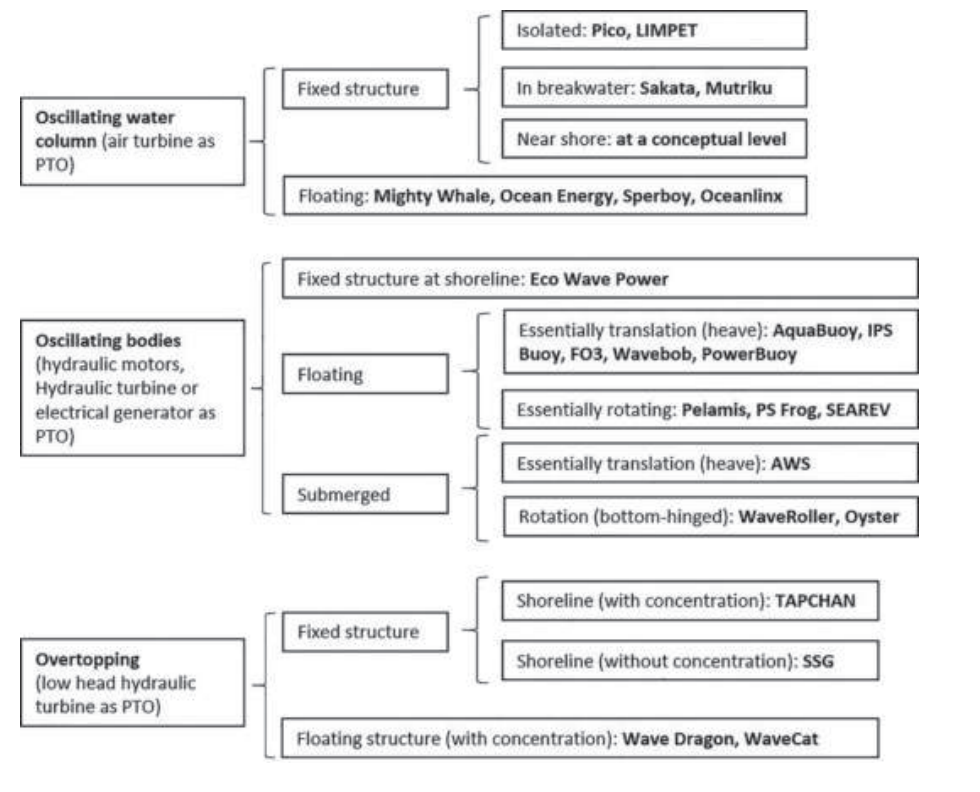
\includegraphics[scale=0.6]{Technologies.png}
	\caption{Wave energy technology}
\end{figure}


\end{document}